\documentclass[9pt,a9paper,handout]{beamer}
\usepackage[utf8]{inputenc}
\usepackage[francais]{babel}
\usepackage[T1]{fontenc}
\usepackage{amsmath,amsfonts,amssymb,tikz,colortbl,lmodern,xspace,subfigure}
\usepackage{tikz}

\definecolor{c979797}{RGB}{151,151,151}
\definecolor{cff0000}{RGB}{255,0,0}
\definecolor{c0000ff}{RGB}{0,0,255}

%\usefonttheme{serif}

\usetheme{Berlin}
\usecolortheme{beaver}
\setbeamertemplate{caption}{\raggedright\insertcaption\par}
\setbeamercolor{item projected}{bg=darkred,fg=white}
\beamertemplateballitem

\newcommand{\command}[1]{$\left|\;\;\;\texttt{#1}\right.$}

\title{\textsc{Introduction à Git}}

\author{Club Robotronik Phelma}
\date{10 Décembre 2015}


\defbeamertemplate*{footline}{myfootline}
{
  \leavevmode%
  \hbox{%
  \begin{beamercolorbox}[wd=.32\paperwidth,ht=2.25ex,dp=1ex,left]{title in head/foot}%
    \hspace{4px}Félix Piédallu
  \end{beamercolorbox}%
  \hspace*{-5px}
  \begin{beamercolorbox}[wd=.34\paperwidth,ht=2.25ex,dp=1ex,center]{title in head/foot}%
    \insertshortauthor
  \end{beamercolorbox}%
  \hspace*{-5px}
  \begin{beamercolorbox}[wd=.36\paperwidth,ht=2.25ex,dp=1ex,right]{title in head/foot}%
    \insertshortdate{}\hspace*{2em}
    \insertframenumber{} / \inserttotalframenumber\hspace*{2ex} 
  \end{beamercolorbox}}%
  \vskip0pt%
}

\begin{document}

\begin{frame} \titlepage       \end{frame}
\begin{frame} \tableofcontents \end{frame}

\section{Qu'est-ce que Git ?}
\subsection{Un gestionnaire de versions}
\begin{frame}
\frametitle{Qu'est-ce que Git ?}
\framesubtitle{Un gestionnaire de versions}
\begin{itemize}
    \item Faire des test sans crainte
    \item Conserver une version toujours fonctionnelle
    \item Travailler en commun
    \item \textbf{Fusionner des modifications automatiquement}
    \item Travailler chacun dans son coin (train…) sans risque de conflits à l'arrivée
\end{itemize}
\end{frame}

\begin{frame}
\begin{itemize}
    \item Utilisation basique très simple à apprendre
    \begin{itemize}
        \item \texttt{git clone https://github.com/robotronik/git-initiation}
        \item \texttt{git add / rm <fichiers>}
        \item \texttt{git commit -m "message"}
        \item \texttt{git pull / push}
        \item Création de branches
    \end{itemize}
    \item Utilisation avancée plus complexe mais très puissante
    \begin{itemize}
        \item \texttt{git merge / rebase}
        \item \texttt{git filter-branch}
        \item Retourner dans le passé et réutiliser d'anciennes modifications
        \item \texttt{git -\,-prune} (soyons fous)
    \end{itemize}
\end{itemize}
\end{frame}

\subsection{À quoi peut ressembler un historique sur Git ?}
\begin{frame}
\frametitle{}{À quoi peut ressembler un historique sur Git ?}
\begin{figure}
    \begin{center}
        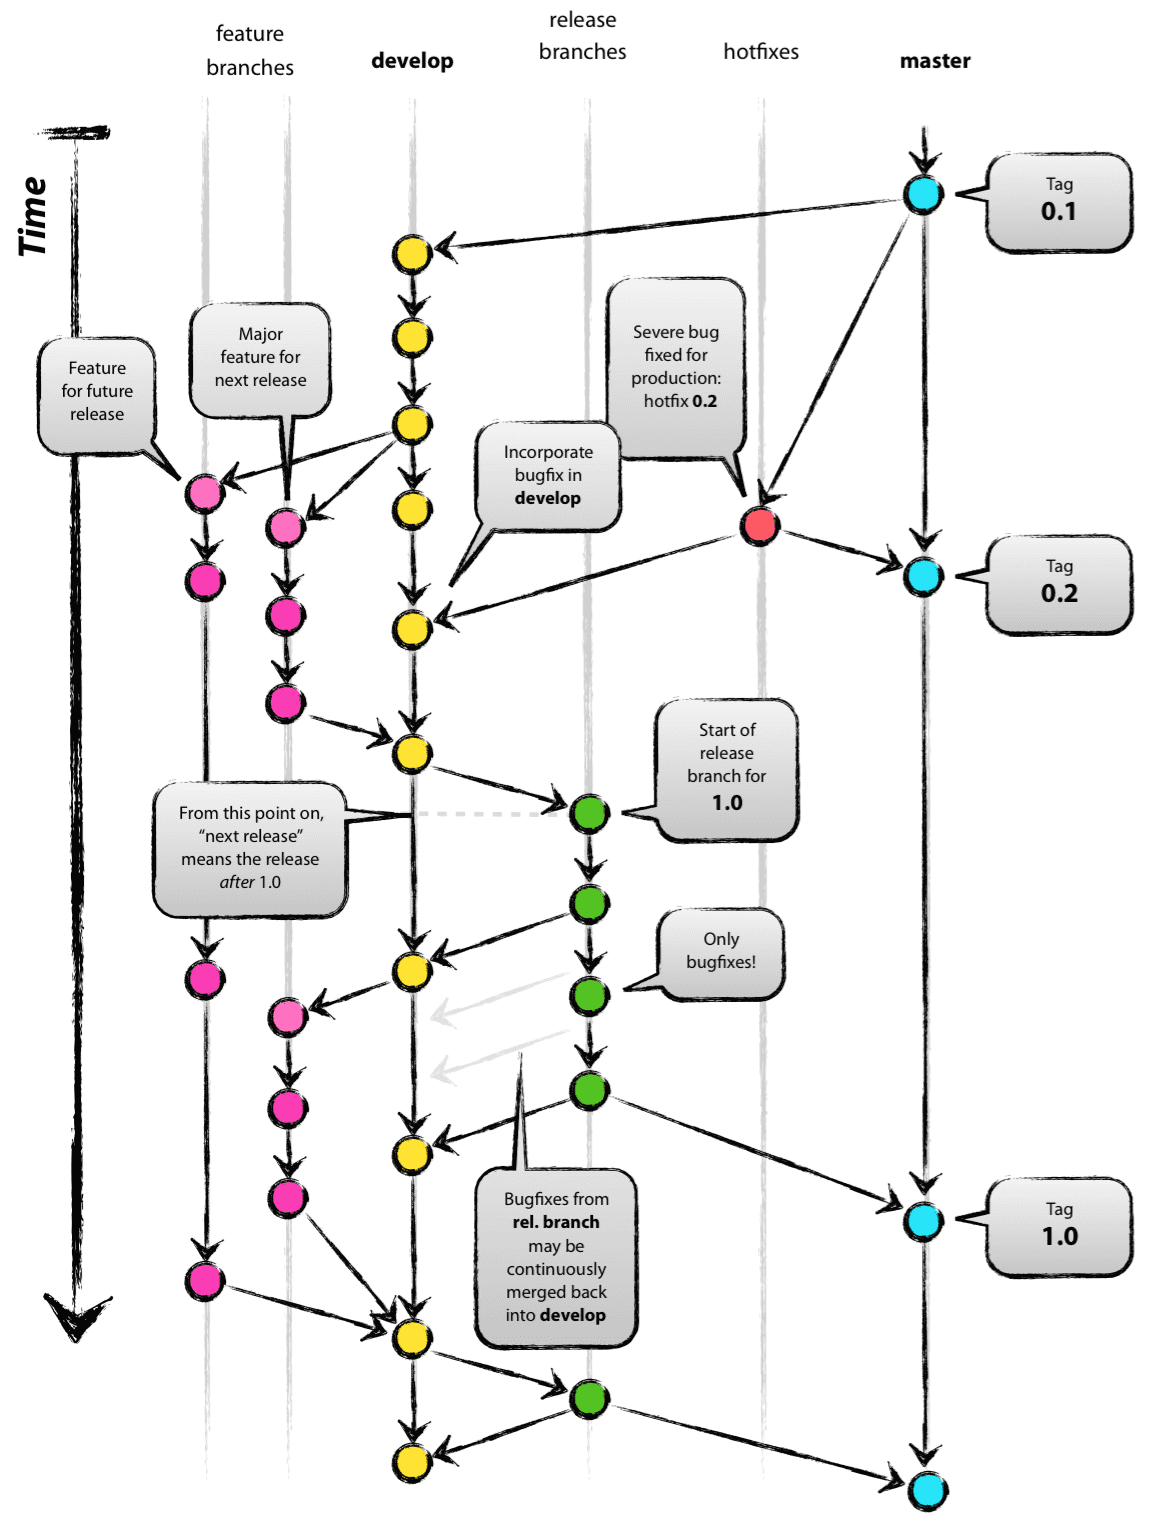
\includegraphics[height=0.7\textwidth]{git-tree}
    \end{center}
\end{figure}
\end{frame}

\section{Commandes basiques}
\subsection{Récupérons un dépôt}
\begin{frame}
\frametitle{Passons à la pratique !}
\begin{itemize}
    \item Récupérons le dépôt\\\command{git clone https://github.com/robotronik/git-initiation}
    \item Regardons son état et son historique\\
    \command{git status}\\
    \command{git log -{}-graph -{}-all}
\end{itemize}
\end{frame}

\subsection{Personnalisation de Git}
\begin{frame}
\frametitle{Personnalisation de Git}
\texttt{\# Nécessaires :\\
git config -{}-global user.name "<votre nom>"\\
git config -{}-global user.email <votre\_adresse@mail>\\
\# Non nécessaires :\\
git config -{}-global core.editor <éditeur\_préféré>\\
git config color.ui auto\\
\# (permet d'avoir une coloration dans le terminal, pas de base à phelma)
}
\end{frame}

\subsection{Création d'une branche}
\begin{frame}
\frametitle{Création d'une branche}
Cela permet de travailler sur une fonctionnalité sans se soucier des autres.
\begin{itemize}
    \item Basculer sur une branche déjà existante :\\
        \command{git checkout felix/localisation}
    \item Créer une nouvelle branche :\\
        \command{git checkout -b moi1A/ma\_branche}
    \item Lister les branches :\\
        \command{git branch -a}
\end{itemize}
\end{frame}

\subsection{Création et modification de fichiers}
\begin{frame}
\frametitle{Création et modification de fichiers}
On va ajouter ou modifier des fichiers du dépôt.
\begin{itemize}
    \item Signaler à git les modifications :\\
    \command{git add monfichier}\\
        on peut faire "\texttt{git add *}" mais peu recommandé\\
        on peut faire "\texttt{git add .}" si le fichier n'est pas nouveau mais modifié\\
    \item On "commit" les modifications :\\
        \command{git commit -m "j'ai ajouté un fichier"}\\
        on peut faire "\texttt{git commit -am}", si il n'y a pas de modifications \\(et alors pas besoin de git add)
    \item On peut corriger le précédent commit (tant qu'il est en local) :
        \command{git commit -{}-amend}
\end{itemize}
\end{frame}


\subsection{Les messages de commit}
\begin{frame}
\frametitle{Les messages de commit}
Ils sont d'une importance capitale !\\

Ils nous permettent de retrouver 6 mois plus tard… Comment on a résolu ce bug déjà ?\\

Ils doivent être courts (= une ligne = 80 caractères), mais si il faut détailler, on peut dépasser :D
\end{frame}


\section{Travailler avec les autres}
\begin{frame}
\frametitle{Travailler avec les autres}
\begin{itemize}
    \item Envoyer ses commits : \\\command{git push}
    \item Récupérer les commits distants : \\\command{git pull}\\
    \item Ceci va merger (fusionner), il est possible de juste récupérer sans merger :\\\command{git fetch}
    \item On peut ensuite merger à la main :\\\command{git merge}
\end{itemize}
\end{frame}

\section{Le fichier .gitignore}
\begin{frame}
\frametitle{Le fichier .gitignore}
\begin{itemize}
    \item Permet d'ignorer des fichiers
    \item Très utile pour les fichiers générés ou la configuration des logiciels
    \item Est présent à la racine de chaque dépôt
\end{itemize}
\end{frame}

\section{La cachette (stash)}
\begin{frame}
\frametitle{La cachette (stash)}
Elle permet de "cacher" les modifications de git (les déplacer dans un coin). Comme ça on peut pull, merge, etc, puis \emph{ensuite} les ressortir et gérer les conflits (eh oui :(… )
\begin{itemize}
    \item "Cacher" les modifications\\\command{git stash}
    \item Ressortir les modifications\\\command{git stash pop}
    \item Détruire le stash\\\command{git stash drop}
\end{itemize}
\end{frame}


















\begin{frame}
    \frametitle{\textsc{À vous de jouer  !}}
    \begin{center}
    \Large \textbf{C'est tout pour aujourd'hui !\\ N'hésitez pas à poser vos questions aux anciens ;) }
    \end{center}
\end{frame}
\end{document}


        \item \texttt{git add / rm <fichier>} : Suivre ou supprimer des fichiers\vspace*{2mm}
        \item \texttt{git commit} : Une "étape", nécessite un message explicite\\("ajouté telle fonctionnalité", "résolu tel bug")\vspace*{2mm}
        \item \texttt{git pull / push}



